\icode[magenta]{E-MCH-SI-L4-261026-001}
如图所示，从固定在水平地面上的斜面顶端\(A\)点朝不同方向抛出两个初速度大小相同的小球(可视为质点)，两小球恰能落在斜面上的同一点\(B\)，两小球运动的时间分别为\(t_1\)、\(t_2\)，若要使小球以最小的初速度从\(A\)点抛出并落到\(B\)点，不计空气阻力，则该小球运动的时间为\paren[]

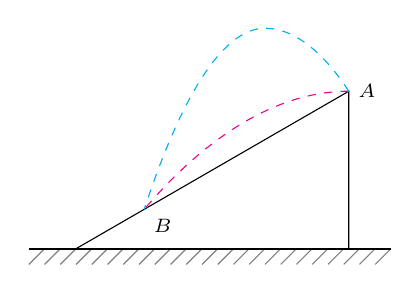
\begin{tikzpicture}[font=\scriptsize]
	\draw (0,0)--(30:4)--({2*sqrt(3)},0);
	\draw[dashed,magenta] (30:4)node[right,black]{\(A\)} parabola bend(30:4)(30:1);
	\draw[dashed,cyan] (30:4) parabola bend(2.4,2.8)(30:1);
	\node at(30:1)[below right]{\(B\)};
	\foreach \x in {-.6,-.4,...,4}
		\draw[gray] (\x,-.2)--++(.2,.2);
	\draw[thick] (-.6,0)--(4,0);
\end{tikzpicture}
\begin{choices}
	\item \(\sqrt{\frac{t_1^2 + t_2^2}{2}}\)
	\item \(\frac{t_1 + t_2}{2}\)
	\item \(\sqrt{t_1t_2}\)
	\item \(\frac{2t_1t_2}{t_1 + t_2}\)
\end{choices}
\begin{answer}
    
\end{answer}